\documentclass[11pt,a4paper,bibliography=totocnumbered,listof=totocnumbered]{scrartcl}
\usepackage[english]{babel}
\usepackage[utf8]{inputenc}
\usepackage{amsmath}
\usepackage{nameref}
\usepackage{amsfonts}
\usepackage{amssymb}
\usepackage{float}
\usepackage{graphicx}
\graphicspath{{Figures//}} % Specifies the directory where pictures are stored
\usepackage{fancyhdr}
\usepackage{tabularx}
\usepackage{geometry}
\usepackage{setspace}
\usepackage[right]{eurosym}
\usepackage[printonlyused]{acronym}
\usepackage{subfig}
\usepackage{floatflt}
\usepackage[usenames,dvipsnames]{color}
\usepackage{colortbl}
\usepackage{color}
\usepackage{paralist}
\usepackage{array}
\usepackage{titlesec}
\usepackage{parskip}
\usepackage[right]{eurosym}
\usepackage[subfigure,titles]{tocloft}
\usepackage[pdfpagelabels=true]{hyperref}
\usepackage{units}
\usepackage{booktabs}
\usepackage{listings}
\usepackage{bold-extra}
\usepackage{pythonhighlight} % python highlighting
\lstset{mathescape=true,
        %frame=tB,
        numbers=left, 
        numberstyle=\tiny,
        basicstyle=\ttfamily\footnotesize, 
        numbers=left,
        morekeywords={Input, for, in},
        keywordstyle = \bfseries,
        xleftmargin=.04\textwidth, 
        captionpos=b,
        breaklines=true, 
        showstringspaces=false, 
        tabsize=2, 
        frame=shadowbox}
\renewcommand{\lstlistingname}{Algorithmus}% Listing -> Algorithm
\captionsetup[lstlisting]{font={small}}
\makeatletter
\def\l@lstlisting#1#2{\@dottedtocline{1}{0em}{1em}{\hspace{1,5em} Lst. #1}{#2}}
\makeatother

\geometry{a4paper, top=25mm, left=20mm, right=20mm, bottom=25mm, headsep=10mm, footskip=12mm}

\hypersetup{unicode=false, pdftoolbar=true, pdfmenubar=true, pdffitwindow=false, pdfstartview={FitH},
	pdftitle={Ausarbeitung Evolutionsstrategien als Alternative zu Bestärkendem Lernen im Bereich der Künstlichen Intelligenz},
	pdfauthor={Daniela Schacherer},
	pdfsubject={Seminararbeit},
	pdfcreator={\LaTeX\ with package \flqq hyperref\frqq},
	pdfproducer={pdfTeX \the\pdftexversion.\pdftexrevision},
	pdfkeywords={Seminararbeit},
	pdfnewwindow=true,
	colorlinks=true,linkcolor=black,citecolor=black,filecolor=magenta,urlcolor=black}
\pdfinfo{/CreationDate (D:20110620133321)}
\newcommand*{\quelle}{%
  \footnotesize Quelle:
  }

\begin{document}

\titlespacing{\section}{0pt}{12pt plus 4pt minus 2pt}{-6pt plus 2pt minus 2pt}

% Kopf- und Fusszeile
\renewcommand{\sectionmark}[1]{\markright{#1}}
\renewcommand{\leftmark}{\rightmark}
\pagestyle{fancy}
\lhead{}
\chead{}
\rhead{\thesection\space\contentsname}
\lfoot{}
\cfoot{}
\rfoot{\thepage}
\renewcommand{\headrulewidth}{0.4pt}
\renewcommand{\footrulewidth}{0.4pt}

% Vorspann
\renewcommand{\thesection}{\Roman{section}}
\renewcommand{\theHsection}{\Roman{section}}
\pagenumbering{Roman}

% %----------------------------------------------------------------------------------------
%	TITLE PAGE
%----------------------------------------------------------------------------------------

\begin{titlepage}

\newcommand{\HRule}{\rule{\linewidth}{0.5mm}} % Defines a new command for the horizontal lines, change thickness here

\center % Center everything on the page

\LARGE Ruprecht-Karls-University Heidelberg \\[0.5cm] % Name of your university/college
\Large Faculty of Math and Computer Science \\[1.5cm]
\Large \textbf{Lecture} Artifical Intelligence \\[0.5cm] % Major heading such as course name

\HRule \\[0.4cm]
{ \textsc{\huge \bfseries An Autocompletion Algorithm using Recurrent Neural Networks}}\\ \textsc{\Large Final project of the lecture }\\[0.4cm] % Title of your document
\HRule \\[1.5cm]

\begin{minipage}{0.4\textwidth}
\begin{flushleft} \large
\emph{Author:}\\
Daniela Schacherer \\% Your name
\end{flushleft}

\begin{flushleft} \large
\emph{Lecturer:}\\
Prof. Dr. Ommer\\ % Your name
\end{flushleft}

\begin{flushleft} \large
\emph{Date:}\\
09.02.2018 \\% Your name
\end{flushleft}

\end{minipage}
~
\begin{minipage}{0.4\textwidth}
\end{minipage}\\[4cm]

\vfill % Fill the rest of the page with whitespace

\end{titlepage}

%----------------------------------------------------------------------------------------
%	INHALTSVERZEICHNIS
%----------------------------------------------------------------

\tableofcontents % Include a table of contents

\newpage % Begins the essay on a new page instead of on the same page as the table of contents 


% ----------------------------------------------------------------------------------------------------------
% Inhalt
% ----------------------------------------------------------------------------------------------------------
% Abstände Überschrift
\titlespacing{\section}{0pt}{12pt plus 4pt minus 2pt}{-6pt plus 2pt minus 2pt}
\titlespacing{\subsection}{0pt}{12pt plus 4pt minus 2pt}{-6pt plus 2pt minus 2pt}
\titlespacing{\subsubsection}{0pt}{12pt plus 4pt minus 2pt}{-6pt plus 2pt minus 2pt}

% Kopfzeile
\renewcommand{\sectionmark}[1]{\markright{#1}}
\renewcommand{\subsectionmark}[1]{}
\renewcommand{\subsubsectionmark}[1]{}
\lhead{Chapter \thesection}
\rhead{\rightmark}

\onehalfspacing
\renewcommand{\thesection}{\arabic{section}}
\renewcommand{\theHsection}{\arabic{section}}
\setcounter{section}{0}
\pagenumbering{arabic}
\setcounter{page}{1}

% ----------------------------------------------------------------------------------------------------------
% Abstract
% ----------------------------------------------------------------------------------------------------------

\section{Abstract}
We are surrounded by artifical intelligent systems that have been developed to ease our everyday lives. One of the areas where such systems have proofed to be very useful is text processing. Features such as auto-completion are meanwhile integrated in every smartphone. \\
In the context of our project, we developed a text auto-completion and prediction system. For that purpose, we built a neural network, suggesting the following character given a prefix. This model will be used to suggest possible word-endings and generate own texts.
\cite{Chung-et-al-TR2014}
% ----------------------------------------------------------------------------------------------------------
% Introduction
% ----------------------------------------------------------------------------------------------------------
\section{Introduction}

Neural networks are a very popular solution to classification problems.
Assumed that the given task is to distinguish pictures of different animals like for instance a cat, a dog, a zebra and an elephant. A classical feedforward network can easily be trained to classify a given picture into one of the learned categories and it can also solve that task for the following pictures. This is the case because there is no relation between the previous and the current output, meaning that the output at time $t$ is independent of the output at time $t-1$. \\
However there are some scenarios where the previous output is needed in order to get the new output, for example when dealing with sequences like text, genomes or numerical time series data. In such a case a meaningful prediction e.g. predicting the next character can only be made based on the current and one or multiple previous outputs e.g. knowing a specified number of preceding characters.


\subsection{Recurrent neural networks}
In such a case like the one mentioned above \textbf{recurrent neural networks} (RNN) are the method of choice. Figure 1 displays the architecture of a simple RNN. Each of the unrolled network states $A$ receives the current input $x_t$ as well as the input at time $t-1$ and computes the ouput considering both. More precisely the network first calculates the hidden state $h^{(t)}$ at time $t$ using the current input $x_t$ and the previous hidden state $h^{(t-1)}$ each multiplied by the respective weight matrix, adds a bias $b_h$ and applies a specific function $g_h$ to it. After that the current output $y^{(t)}$ is derived from the hidden state $h^{(t)}$. 
\begin{align*}
	a^{(t)} &= g_h(w_i x^{(t)} + w_R a^{(t-1)} + b_h) \\
	h^{(t)} &= g_y(w_y a^{(t)} + b_y)
\end{align*} 

% include a picture
	\begin{figure}[h!] 
	\begin{minipage}{\textwidth}
     \centering
		\center{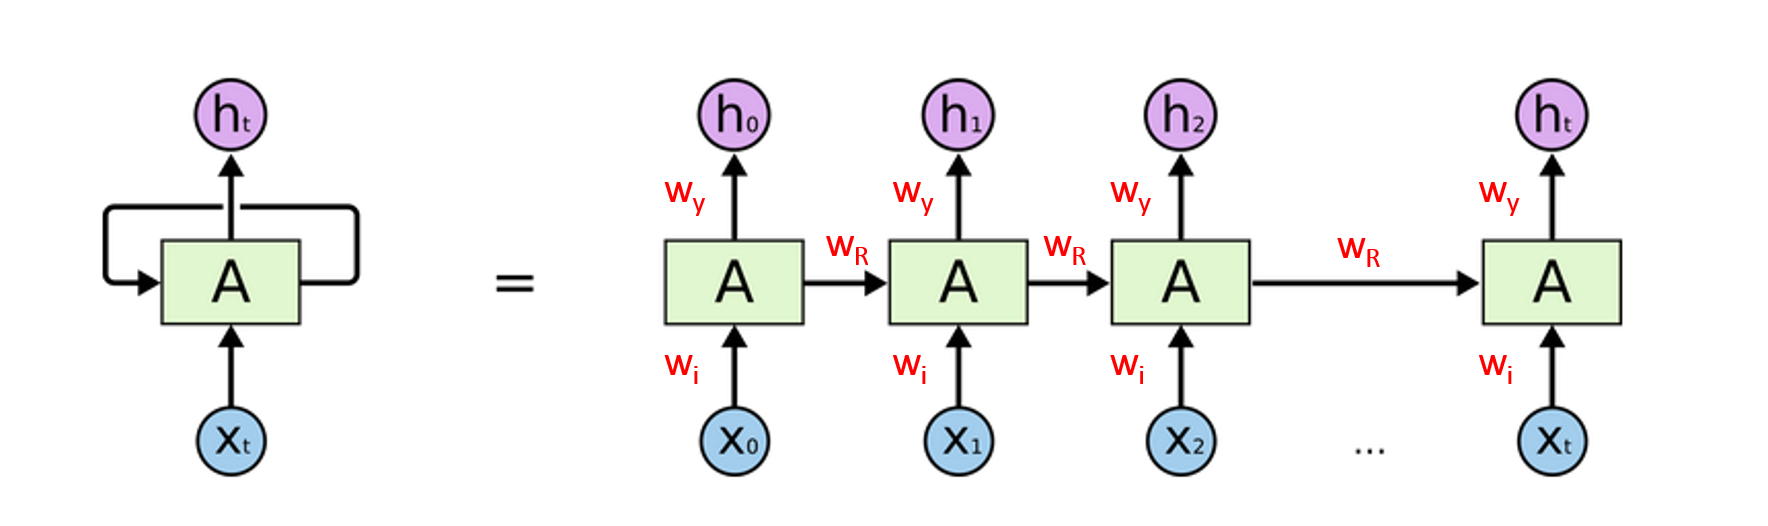
\includegraphics[width=0.7\linewidth]{rnn2}}
		\label{fig:rnn0}
		\caption{An unrolled recurrent neural network. Source: \textit{http://colah.github.io/posts/2015-08-Understanding-LSTMs/}}
	\end{minipage}
	\end{figure}

RNNs like the ones above can apparently \glqq memorize \grqq the information from the timepoint directly before the current time. However, there are also situations where the information from even earlier timesteps is needed for the prediction. The necessity of remembering information for long time periods is also referred to as long-term dependencies. For learning them,  a special kind of RNN which is called the \textbf{Long Short Term Memory Network} (LSTM) is needed \cite{Goodfellow-et-al-2016, lstm_colah}.

\subsection{Long Short Term Memory Networks}
The concept of LSTMs was first introduced in 1997 by Hochreiter \& Schmidhuber \cite{hochreiter1997long} in order to tackle the problem of long-term dependencies.  
In comparison to RNNs, LSTMs have a more complex repeating module each consisting of four interacting layers. 
Figure 2 depicts this module. The central part of an LSTM is the straight horizontal line, called the cell state $C$. There are three \textbf{gates} that enable to add (\glqq memorize \grqq) or remove (\glqq forget \grqq) information from the cell state. 

% include a picture
	\begin{figure}[H] 
		\center{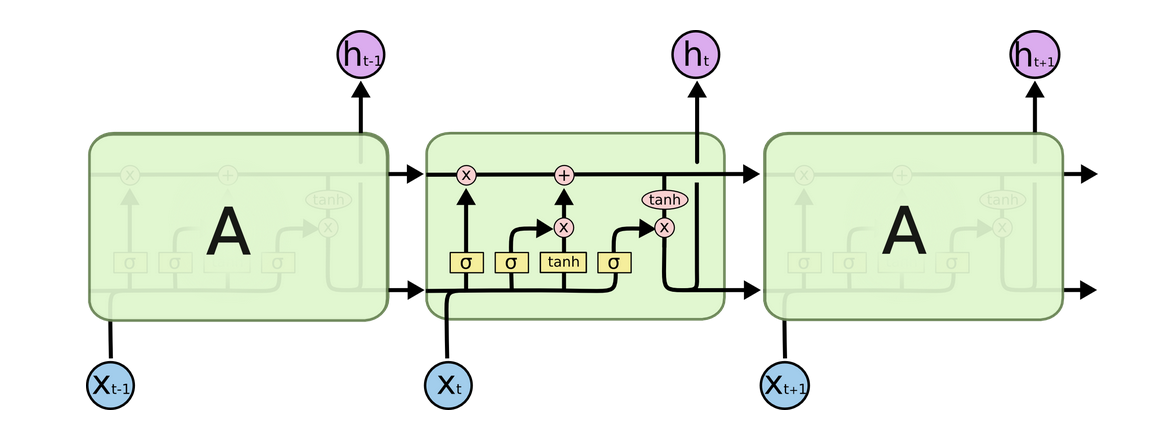
\includegraphics[width=0.5\linewidth]{lstm}}
		\label{fig:cell_state}
		\caption{Architecture of an LSTM module. Source: \textit{http://colah.github.io/posts/2015-08-Understanding-LSTMs/}}
	\end{figure}

The forget gate controls which part of previous output $h_{t-1}$ and current input $x_t$ will be removed from the cell state. Practically the forget gate is a sigmoid layer providing a vector of numbers between 0 and 1, which will determine for every number in the cell state how much information is kept (0 - forget everything; 1 - keep everything).

% include a picture
	\begin{figure}[h!] 
		\center{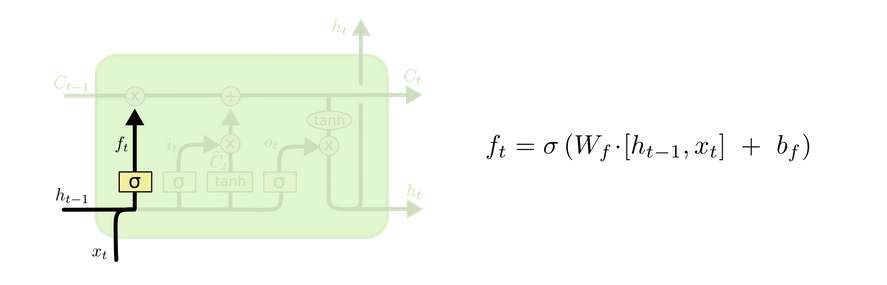
\includegraphics[width=0.5\linewidth]{forget}}
		\label{fig:forget}
		\caption{The forget gate. Source: \textit{http://colah.github.io/posts/2015-08-Understanding-LSTMs/}}
	\end{figure}

In order to add new information to the cell state, two steps are performed. First, a tanh layer creates a vector of new values $\tilde{C_t}$. Following this another sigmoid layer - also referred to as input gate - determines how much of the corresponding $\tilde{C_t}$ value is added to the cell state.

% include a picture
	\begin{figure}[h!] 
		\center{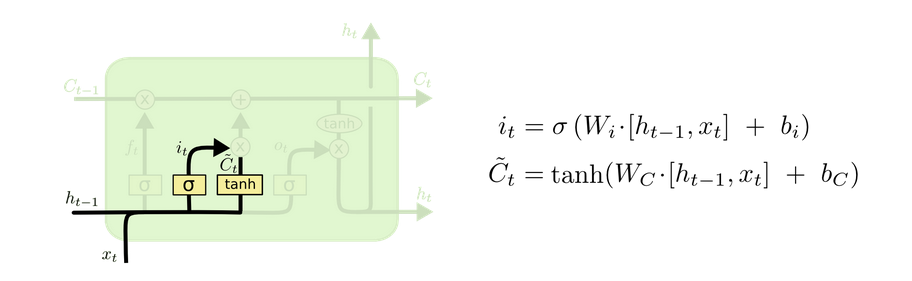
\includegraphics[width=0.5\linewidth]{input}}
		\label{fig:input}
		\caption{The input gate. Source: \textit{http://colah.github.io/posts/2015-08-Understanding-LSTMs/}}
	\end{figure}

Based on these operations the cell state $C_{t-1}$ can be updated to $C_t$ by forgetting (multiplying the previous cell state by $f_t$) and adding (multiplying the candidate values $\tilde{C}_t$ with $i_t$). 
\begin{align*}
	C_t = f_t \cdot C_{t-1} + i_t \cdot \tilde{C}_t
\end{align*}

Finally the output $h_t$, which is not equal to the cell state, but rather a filtered version of it, is computed at the output gate. For example if considering a language model, the cell state could contain information about a subject and the network wants to predict the following verb. The output $h_t$ could then be simply determined from whether the subject is singular or plural providing information about how the predicted verb should be conjugated. \\
To compute the output a sigmoid layer and a tanh layer are used to decide which parts of the cell state should be contained in the output \cite{Goodfellow-et-al-2016, lstm_colah}.

% include a picture
	\begin{figure}[h!] 
		\center{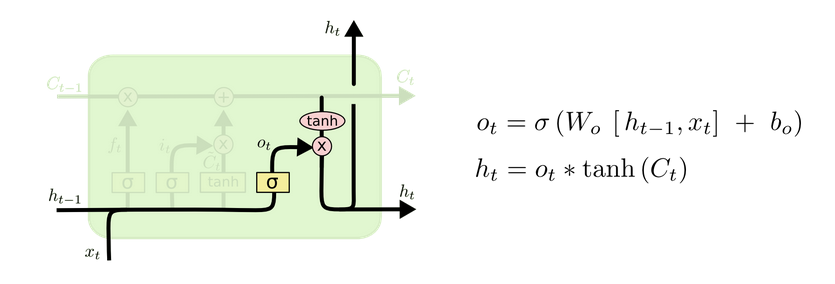
\includegraphics[width=0.5\linewidth]{output}}
		\label{fig:output}
		\caption{The output gate. Source: \textit{http://colah.github.io/posts/2015-08-Understanding-LSTMs/}}
	\end{figure}

\subsection{Gated recurrent unit}
The idea behind a gated recurrent unit (GRU) layer is very similar to that of a LSTM layer, although there are a few differences. There are only two gates (reset and update gate)  in a GRU instead of three in a LSTM. Also a GRU does not possess an internal cell state $c$ which is different from the hidden state $h$. The reset gate $r$ basically describes how to combine the current input and the previous hidden state, while the update gate $z$ defines how much of the previous hidden state is taken into account for calculating the output. Using these two gates the current hidden state $h_t$ can be calculated \cite{gulli2017deep}. 
\begin{align*}
	r_t &= \sigma(W_r [h_{t-1},x_t] + b_r) \\
	z_t &= \sigma(W_z [h_{t-1},x_t] + b_z) \\
	n_t &= \tanh(W_{in} x_t + b_{in} + r_t \cdot (W_{hn}H_{t-1} + b_{hn})) \\
	h_t &= (1-z_t) \cdot n_t + z_t \cdot h_{t-1}
\end{align*}

\pagebreak


%
%----------------------------------------------------------------------------------------------------------
% Programming
% %----------------------------------------------------------------------------------------------------------
\section{Methods}
In general, the implementation was done in many group sessions including all group members. 
Within the scope of the project, we tried to assign subtasks to each member. While Marvin Klaus made greater effort in implementing the GUI, Daniela Schacherer concentrated on Data Preprocessing and network architecture and Sebastian Bek was assigned to the task of specific hyperparemter optimization and evaluation. 

\subsection{Requirements}
We used the programming language python version 3.6 and pytorch version 0.2.0-4 as the framework to implement the neural network. 

\subsection{Data Preprocessing \small{(woman in charge: Daniela Schacherer)}}
As traininig data we use Friedrich Nietzsche’s \textit{Beyond Good and Evil} which is available as a free of charge e-book via http://www.gutenberg.org. \\
The complete text has a length of $181124$ characters and we use the first half of it to generate our training samples, while the second half was dedicated as test set. We make the complete text lower case and remove all special characters like for instance commas, points and quotation marks. \\
To generate our training set we split the preprocessed text into slices of 100 characters spacing the sequences by an offset of 1 character. By this we yield a total of 64000 training instances (features). Additionally, the 101st character which we aim to predict is stored as well. \\
The features are then converted into one-hot encoded vectors. One hot encoding uses one boolean column for each of the classes that in our case correspond to the unique characters. Naturally only one of these columns can take the value 1 (= true) for one sample. Thus, for one sentence we obtain an one hot encoding with dimension \textit{sequence length} $\times$ \textit{number of classes}.

% include a picture
	\begin{figure}[h!] 
		\center{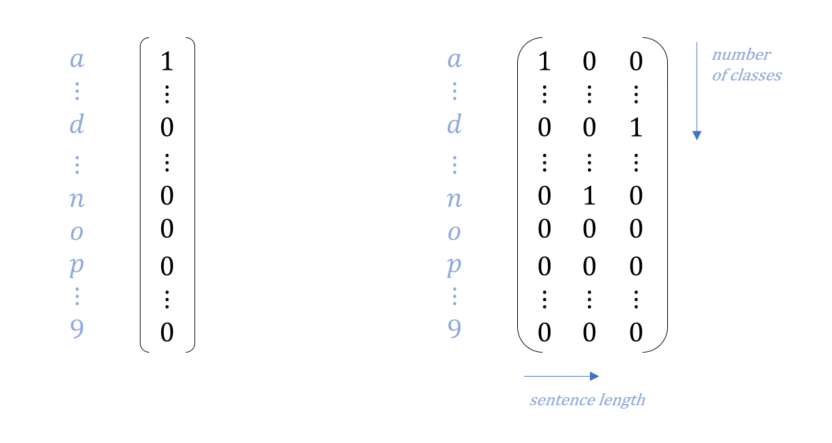
\includegraphics[width=0.5\linewidth]{onehot}}
		\label{fig:onehot}
		\caption{Example for an one hot encoding. Left: One hot encoding of the letter \textit{a}. Right: One hot encoding of the word \textit{and}. The encoding dimensions are \textit{sequence length} $\times$ \textit{number of classes}.}
	\end{figure}

\subsection{Network Architecture \small{(woman in charge: Daniela Schacherer)}} \label{ssec:na}
Our network consists of a gated recurrent unit (GRU) layer, which mainly differs from a classical LSTM layer by having only two gates (reset and update gate) instead of three (input, output and forget gate). According to GRU units perform as well as LSTMs in language modelling tasks while being computationally more efficient. We use a two-layer GRU architecture each layers consisting of 256 neurons i.e. hidden size = 256. The GRU layers are followed by a fully connected layer with as many neurons as unique characters exist in our text. \\
The input to the network is an one-hot encoding of size \textit{sentence length} $\times$ \textit{batch size} $\times$ \textit{number of classes}. In contrast to classification tasks, where only the last output of an LSTM/GRU layer is used, we are making a prediction at every step, so we are as well calculating loss at every step. This is also referred to as multistep loss calculation (cf. multi-step loss/teacher forcing). In practice this means that we iterate over every character in a sentence, let the network predict the following character, calculate the loss regarding this prediction and add it to a total loss variable until we eventually make an update step. This approach turned out to be crucial for the network to perform reasonably.

\subsection{Parameters \small{(man in charge: Sebastian Bek)}}
One of the main challenges during this project apart from defining the network architecture was to find convenient settings regarding the loss function, the optimizer type as well as the values for parameters like for instance the learning rate.  
\begin{itemize}
	\item \textbf{Loss function}: As we needed a categorial class measure we decided to use the torch.nn.CrossEntropyLoss which combines a LogSoftMax and the Negative Log Likelihood Loss in one single class. 
	\begin{align*}
		Loss(x, class) = -log \left( \frac{exp(class)}{\sum_j exp(x_j)} \right)
	\end{align*}	 

	\item \textbf{Optimizer}: By trial and error we found that the Adam optimizer torch.optim.Adam performed best. This optimizer implements the Adam algorithm which is an extension of the stochastic gradient algorithm using adaptive per-parameter learning rates instead of one fixed learning rate for all network parameters. 
	
	\item \textbf{Further parameters}: By separate testing (see \nameref{sec:res}) we found a value of 0.0004 up to 0.0075 for the learning rate, a batch size of 512 and a hidden size (number of neurons in the GRU layer) of 256 to be suitable to our scenario. 
\end{itemize}

The \textit{hidden\_ size} (number of hidden units\/ nodes) parameter can be interpreted as the DOFs ($=$degrees of freedom) of the network. If it is set too low, the model is unable to learn reasonably, since its complexity is too low to capture the predictive factors. Generally, an increased hidden size leads to faster learning but also to faster overfitting (unability to generalize), in case it is set to high. The \textit{num\_ layers} parameter defines how many GRU layers are stacked on top of another. Increasing it to 2, leads to a more powerful network with an increased generalization ability and hence an increased accuracy, but further increasing leads again to too many degrees of freedom, which results in overfitting. Increasing the \textit{batch\_ size} parameter leads to higher computational efficiency, but also to slower learning/converging to a solution. A higher \textit{seq\_ len} is forcing a more content-based prediction. A higher sequence length uses more timesteps and thus more content for prediction.

\subsection{Visualization \small{(man in charge: Marvin Klaus)}}
We also implemented a GUI to provide an interactive interface to our autocompletion network.  

\pagebreak

%
%----------------------------------------------------------------------------------------------------------
% Results
% %----------------------------------------------------------------------------------------------------------
\section{Results} \label{sec:res}

\subsection{Training and testing performance}
The training performance of our network is monitored as the total cross entropy loss of all sample batches divided by the length of the training and the sequence length (the latter in order to account for the multistep loss). The testing performance is measured as the loss of the predicted character and the ground truth (target) normalized over the whole test set. 


% include a picture
\begin{figure}[H]
   \begin{minipage}{\textwidth}
     \centering
     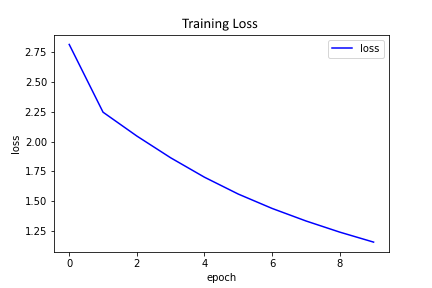
\includegraphics[width=.4\textwidth]{loss_train_hs256_slow}
     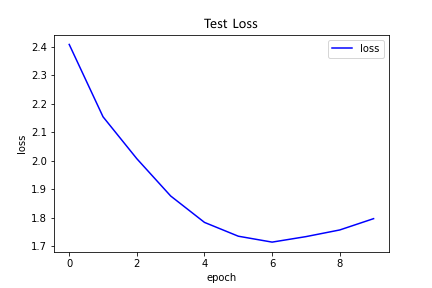
\includegraphics[width=.4\textwidth]{loss_test_hs256_slow}
     \caption{Training of the network was performed using a two-layer GRU, a learning rate of $0.0004$, a batch size of $512$ and a hidden size of $256$. Input sequence length was 100 characters. The left image shows the training loss while the right figure displays the loss during testing.}
     \label{fig:loss1}
   \end{minipage}\\[1em]   
\end{figure}

As can be inferred from figure \ref{fig:loss1} we were able to depress the loss to $1.2$ after $8$ epochs of training using the following settings
\begin{itemize}
	\item learning rate: $0.0004$
	\item batch size: $512$
	\item hidden size: $256$
	\item sequence length of training and test samples: 100 characters
\end{itemize}
The test loss reaches its minimum of $1.7$ in epoch $6$ and then starts to increase again. This indicates that overfitting to the training data is occuring from then on (compare figure \ref{fig:stop}). As we want to avoid this phenomenon in the first place, we stop the training and save the network parameters after the $6$th training epoch. However, if the network is applied for text generation overfitting is desired which is why we use a different number of training epochs for this task (see section \ref{ssec:tg}).

% include a picture
\begin{figure}[H]
   \begin{minipage}{\textwidth}
     \centering
     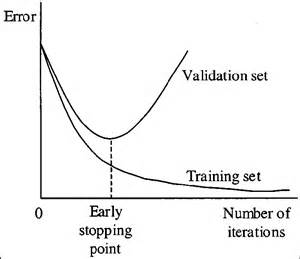
\includegraphics[width=.4\textwidth]{early-stopping-graphic}
     \caption{Schematic of a neural network training with early stopping. The network is repeatedly trained as long as the error on the test set (test error) is on the decrease. When the test error starts to increase, the training is halted. Source \textit{https://elitedatascience.com/overfitting-in-machine-learning}}
     \label{fig:stop}
   \end{minipage}\\[1em]   
\end{figure}

\subsection{Determination of the optimal hidden size}
We tested different values for the hidden size i.e. number of neurons in the hidden layer of the GRU, and evaluated them by observing the prediction accuracy on the test set. 
We examine the amount of correctly predicted characters for sequences of length \textit{seqlen}, which are generated analogously to the training samples but originate from the second half of our input text which we dedicated as test text. The ratio of correctly predicted characters is referred to as the accuracy of the network. \\
For this purpose we used a learning rate of $0.001$ instead of $0.0004$ in order to ease observing the long-term behaviour. The figure below shows accuracy plots for a hidden size of $128$ respectively $256$. As we reached a higher prediction accuracy ($51 \%$) using the larger hidden size we fixed this parameter for further testing.  Further increasement of the hidden size only leads to higher computation effort and faster overfitting.

% include a picture
\begin{figure}[!ht]
   \begin{minipage}{\textwidth}
     \centering
     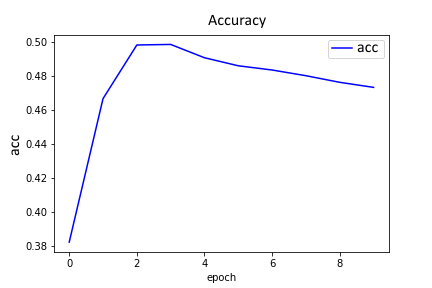
\includegraphics[width=.4\textwidth]{acc_hs128}
     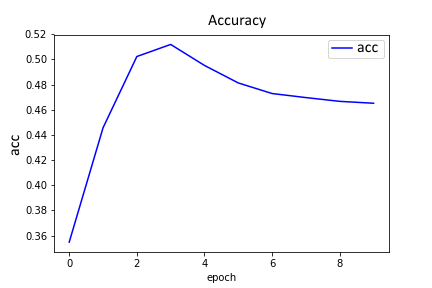
\includegraphics[width=.4\textwidth]{acc_hs256}
     \caption{Prediction accuracy on the test set. Left: Training was performed using a two-layer GRU, a learning rate of $0.001$, a batch size of $512$ and a hidden size of $128$. A maximum accuracy of $49\%$ is reached. Right: Training was performed using a two-layer GRU, a learning rate of $0.001$, a batch size of $512$ but a hidden size of $256$. Here a maximum accuracy of $51 \%$ could be achieved after 3 epochs of training.}
     \label{fig:sub1}
   \end{minipage}\\[1em]   
\end{figure}

\subsection{Prediction performance}
We present the performance evaluation on the two-layer GRU network trained with the following configurations:
\begin{itemize}
	\item learning rate = $0.0004$
	\item batch size = $512$
	\item hidden size = $256$
	\item number of training epochs = $6$
\end{itemize} 

\subsubsection{Prediction of the next character}
How well the network performs, with respect to the task of predicting the next character, is measured as described in the previous section. As the accuracy reaches its maximum at epoch 6, we stopped training and saved the network parameters at this point. 

% include a picture
\begin{figure}[!ht]
   \begin{minipage}{\textwidth}
     \centering
     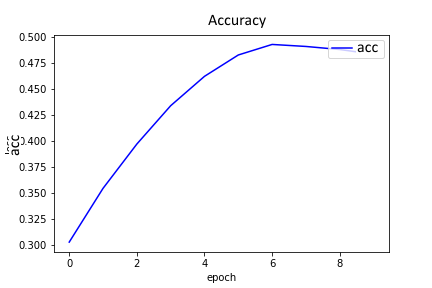
\includegraphics[width=.4\textwidth]{acc_hs256_slow}
     \caption{Prediction accuracy on the test set. Training was performed using a two-layer GRU, a learning rate of $0.0004$, a batch size of $512$ and a hidden size of $256$. A maximum accuracy of almost $50\%$ is reached.}
     \label{fig:truenet}
   \end{minipage}\\[1em]   
\end{figure}

\subsubsection{Prediction of the word ending} \label{ssec:we}
To evaluate the performance of the network at predicting whole word endings we used a quite simple binary approach and checked whether the most probable word ending suggested by our network matches the true word ending in the test text. Although at best $17$ out of $50$ words were completed consistent with the source text, one can observe that many predicted word endings make sense anyway like for instance in the following two cases. \\

\begin{table}[!ht]
\footnotesize
\centering
\begin{tabularx}{\textwidth}{X|X|X}
\textbf{Testcases} & \textbf{GT (ground truth)} & \textbf{predicted string}\\
\toprule 
't does what all nourishment does that does not merely conserveas the phy' & 'siologist' & 'siological' \\
\hline
' of wisdom but rather as disagreeable fools and dangerous inte' & 'rrogatorshave' & 'rpretation' \\ 
\end{tabularx}
	\vskip 1pt
\end{table}

The complete table can be found in the appendix.

\subsection{Text generation} \label{ssec:tg}
To enable the generation of meaningful texts, the network has to be trained with sequences as long as possible. We thus trained the network with sequence length 100 and afterwards let the network produce text given a seed sequence. In contrast to prior prediction tasks we retrained our model for 12 epochs in order to obtain some overfitting as we noticed that this improves the quality of the generated texts. 
The following two example texts were produced by our text generation network given a seed:


\fbox{\begin{minipage}{44em}
seed: \glqq responsibility \grqq \\
...their belief in the habit of interpretation and consequently also a worldexposition and thinks within himself when a thinkers who are still eager for whose sake one afterry that there is nothing little must above all at the value of truth present of its some simply recognize the animal the case in
\end{minipage}}

\fbox{\begin{minipage}{44em}
seed: \glqq psychologist \grqq \\
...s had a natural philosopher his sacrifice for is most developed in places where by a stame that what in the straight of the commander all the greater part of the straight of the commander all the greater part of the straight of the commander all the greater part of the straight of the commander all 
\end{minipage}}

Obviously it is quite difficult to define a quantitative measure of how well the network performs at generating new texts. A human reader can immediately conceive that the generated texts don't make sense regarding content and in the second example the network even starts to repeatedly produce the same sentence fragements. However, every word or smaller text fragment taken individually is reasonable indicating that the text generation would work very well using a network trained with an even higher sequence length or trained with a larger dataset processed with more computational power.


\subsection{Interactive prediction}
algorithmus to generate user definded number of word beginnings. then predict completion.

\pagebreak
%----------------------------------------------------------------------------------------------------------
% Discussion
% %----------------------------------------------------------------------------------------------------------
\section{Discussion}
In summary, we could successfully implement our recurrent neural network and apply it to text autocompletion and text generation tasks. As already mentioned above, finding a suitable network architecture along with an optimal parameter setting turned out to be one of the most time consuming steps within the project. Apart from this problems regarding different operating systems and the lengthy training of the network took a lot of time as well. 

In the end we reached a maximal next-character prediction accuracy of 50\% which is not really convincing at first sight. The word-ending prediction accuracy is even lower than 50\%. However as shown in subsection \ref{ssec:we} it is necessary to take a closer look when dealing with natural language processing tasks. For the analysis of how well word endings are predicted we would thus need a more sensitive measure, which does not simply distinguish between \textit{correct} and \textit{wrong} but takes into account how much sense the word ending makes in the given context. If there was more time for the project this would be a helpful extension in order to assess the quality of such networks. 

The text generation ability of our network turned out to be quite good. It would be interesting to further investigate the sequence length of training samples necessary to produce more meaningful texts. These could then be suitable as chatbots or similar. Also, for the prediction as well as the text generation tasks an even larger training set would possibly lead to a performance growth. For an application of our network in practice, more time and developmental work would be needed. However, with this project we could prove that the task is solvable with moderate computing capacity and within a limited time frame conveniently. 

\pagebreak
\section{Appendix}
\begin{table}[H]
\tiny
\centering
\caption{Word Prediction Test}
\begin{tabularx}{\textwidth}{X|X|X}

Testcases & GT (ground truth) & predicted string\\
\toprule
't everything that we call higher culture is based upon the spiritualising and intensifying ' & 'of' & 'the' \\ 
\hline 
'intevremond who reproached him for ' & 'his' & 'the' \\ 
\hline 
' is no doubt these coming ones will be least able to dispense with the serious and not unscr' & 'upulous' & 'eates' \\ 
\hline 
'amity might be involved ther' & 'ein' & 'e' \\ 
\hline 
'rmula of virtue ' & 'morality' & 'and' \\ 
\hline 
'onsider for ourselves  239 the weaker sex has in no previous age been treated w' & 'ith' & 'ith' \\ 
\hline 
'ose modes of thinking which measure th' & 'e' & 'e' \\ 
\hline 
' home old a dragon thence doth roam  noble titl' & 'e' & 'ed' \\ 
\hline 
't does what all nourishment does that does not merely conserveas the phy' & 'siologist' & 'siological' \\ 
\hline 
'ary courage the standingalone' & ' ' & ' ' \\ 
\hline 
'ed north pole e' & 'xpeditions' & ven \\ 
\hline 
' him only to suffer with his fellows  223 the hybrid europeana tolerably ugly plebeian taken all in ' & 'allabsolutely' & 'the' \\ 
\hline 
'dinganimal alone attains to honours and di' & 'spenses' & 'strust' \\ 
\hline 
'ise woman to defeminize herself in this manner and to imitate all the stupidities from which man in ' & 'europe' & 'the' \\ 
\hline 
'obliged to find' & ' ' & ' ' \\ 
\hline 
's a violation an intentional injuring of the fundamental will of the spirit which instinctive' & 'ly' & ' ' \\ 
\hline 
' things in the old arrangementsin short growth or more properly the' & ' ' & ' ' \\ 
\hline 
' of wisdom but rather as disagreeable fools and dangerous inte' & 'rrogatorshave' & 'rpretation' \\ 
\hline 
'ainful delight of tragedy is cruelty that which operates agreeably in socalled tragic sympath' & 'y' & 'y' \\ 
\hline 
'hearts he would not easily find therein the inten' & 'tion' & 'tion' \\ 
\hline 
'f disguises it enjoys also its feeling of security thereinit is preci' & 'sely' & 'sely' \\ 
\hline 
'ncts there is stupidity in this movement an almos' & 't' & 't' \\ 
\hline 
'ng were proved thereby in favour of woman as she is among men these ' & 'are' & 'precestion' \\ 
\hline 
'what food means and she insists on being coo' & 'k' & 'ure' \\ 
\hline 
' of rank betwee' & 'n' & 'n' \\ 
\hline 
' grandfathers in esteem and also at a little distance from us we europeans of the day after ' & 'tomorrow' & 'the' \\ 
\hline 
'that is a typical sign of shallowmindedness and a thinker ' & 'who' & 'and' \\ 
\hline 
'in our very uncertain and consequently very conciliatory cent' & 'ury' & 'istion' \\ 
\hline 
'the will nothing is so adapted to the spirit of t' & 'he' & 'he' \\ 
\hline 
'selves and what the spirit that leads us wants to be' & ' ' & ' ' \\ 
\hline 
' contemning look the feeling of separation from the multitude with their duti' & 'es' & 'on' \\ 
\hline 
'derstanding of its victimsa repeated pro' & 'of' & 'founder' \\ 
\hline 
' emancipation of woman insofar as it is desired and d' & 'emanded' & 'eception' \\ 
\hline 
'rather a condition of every highe' & 'r' & 'r' \\ 
\hline 
' back in all directions we o' & 'urselves' & 'ne' \\ 
\hline 
'nswer for this diagnosis of the european diseasethe disease of the will is diffused unequally ove' & 'r' & 'r' \\ 
\hline 
'upidities fr' & 'om' & 'om' \\ 
\hline 
'paniard at the sight of the faggot and ' & 'stake' & 'the' \\ 
\hline 
'lfdenial in the religious sens' & 'e' & 'es' \\ 
\hline 
'tes  226 we immoraliststhis world with which we are concerned in which we have ' & 'to' & 'a' \\ 
\hline 
'o other religion is any longer preachedlet the psychologist have his ears open throu' & 'gh' & 'gh' \\ 
\hline 
'ntancespasms to vivisection of conscience and to pascal' & 'like' & 'uation' \\ 
\hline 
'anifold enjoymen' & 't' & 't' \\ 
\hline 
'imperious something which is ' & 'popularly' & 'the' \\ 
\hline 
'reference of ignorance of arbitrary shut' & 'ting' & 'h' \\ 
\hline 
'd blue mocking twilight this aging civilization with ' & 'its' & 'the' \\ 
\hline 
'so many generations must have prepared the way for the coming of the philosopher each of his ' & 'virtues' & 'perhaps' \\ 
\hline 
't its service an apparently opposed impulse of the spirit a sudde' & 'nly' & 'rs' \\ 
\hline 
'ave the hard task and for our recreation gladly seek the company of beings under whose hand' & 's' & ' ' \\ 
\hline 
' the wagnerienne who with unhinged will undergoes the performance of tri' & 'stan' & 't' \\ 
\hline 
\end{tabularx}
   \vskip 1pt
\end{table} 

%----------------------------------------------------------------------------------------------------------
% Literatur
% %----------------------------------------------------------------------------------------------------------


\renewcommand\refname{Literature}
\bibliographystyle{abbrvdin}
\bibliography{bib}
\pagebreak


\end{document}
